\documentclass{beamer}

\usepackage[utf8]{inputenc}
\usetheme{default}

\usepackage{listings}
\lstset{
basicstyle=\small\ttfamily,
columns=flexible,
breaklines=true
}

\usepackage{epstopdf}
\usepackage{multicol}

\makeatletter
\DeclareMathSizes{\f@size}{10}{7}{7}
\makeatother

\title[66.20/86.37]{U.B.A. - Facultad de Ingeniería\\\vspace{0.25cm} 66.20/86.37 Organización de Computadoras
\\Jerarquía de memorias}
\author{Práctica}
\date{1$^{er}$ cuatrimestre 2020}


\begin{document}
\begin{frame}
\titlepage % Print the title page as the first frame
\end{frame}

\begin{frame}
 \frametitle{Introducción}
Características deseadas para un sistema de memoria
    
    \begin{itemize}
      \item La mayor capacidad de memoria posible
      \item La menor latencia posible
      \item El mayor ancho de banda posible
      \item El menor costo posible
      \item El menor consumo de energía, espacio, etc.
    \end{itemize}
    \bigskip
        \textbf{Situación real: cuanto más rápida es una tecnología de memoria,
    más costosa.}
\end{frame}

  \begin{frame}
   
\frametitle{Introducción (cont.)}
    Solución:
    \begin{itemize}
      \item Memoria organizada de forma jerárquica (en varios niveles)
      \item Cada nivel es más rápido, más chico y más costoso por byte que el
      siguiente nivel más bajo
      \item Todos los datos que se encuentran en un nivel dado, se encuentran
      también en los niveles inferiores
    \end{itemize}
    \end{frame}

\begin{frame}
\frametitle{Introducción (cont.)}
    Se busca con esta organización jerárquica:
    \begin{itemize}
      \item Que el costo sea casi tan bajo como el nivel de memoria de menor
      costo.
      \item Que la velocidad sea tan alta como el nivel de memoria más rápido.
    \end{itemize}
    \bigskip

    \textbf{La efectividad de esta solución está dada por los principios de
    localidad espacial y temporal.}
\end{frame}

  \begin{frame}
  \frametitle{Niveles en una jerarquía de memoria}
    \begin{figure}[ht]
    \centering
    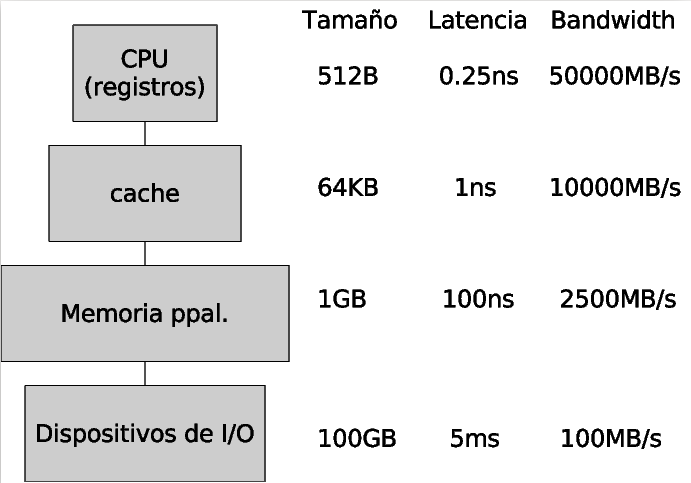
\includegraphics[width=0.9\textwidth]{mh_levels.png}
    \end{figure}
  \end{frame}

  \begin{frame}
   \frametitle{Mejoras performace CPU vs. memoria}
    \begin{itemize}
      \item La mejora de performance en los procesadores fue mucho mayor que en
      las memorias
      \item Esto acrecentó enormemente la importancia de organizar
      jerárquicamente el sistema de memoria (para intentar ``seguirle el paso''
      a las CPUs)
    \end{itemize}

    \begin{figure}[ht]
    \centering
    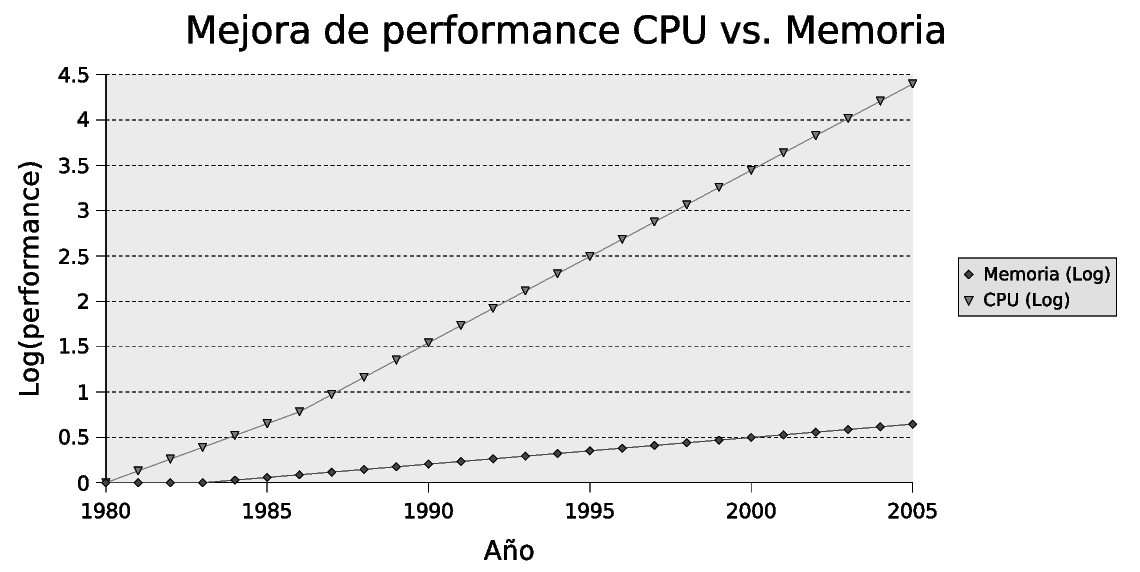
\includegraphics[width=0.7\textwidth]{cpu_mem_perf.png}
    \end{figure}
    \end{frame}

  \begin{frame}
  \frametitle{Latencia y Bandwidth}
    \begin{itemize}
      \item Se busca disminuir la latencia para reducir el tiempo de acceso a
      un dato cualquiera
      \item Se busca aumentar el bandwidth para poder poblar la memoria de nivel
      superior desde la de nivel inferior con la mayor velocidad posible
      \item Un sistema corriendo múltiples procesos simultáneos realiza muchos
      context switches por unidad de tiempo, por lo cual se producirán
      \emph{cache misses} compulsivos (ej: en un server). Este tipo de sistemas
      requieren un gran ancho de banda para poblar rápidamente niveles
      superiores con los datos de los inferiores
    \end{itemize}
  \end{frame}
    
  \begin{frame}
  \frametitle{Caches}
    Cache es el nombre de los primeros niveles de la jerarquía de memoria luego
    de los registros, y antes de la memoria principal (RAM).
    \begin{itemize}
      \item Puede haber varios niveles: L1, L2 y recientemente se introdujo L3
      \item El termino \emph{cache} se utiliza para muchas otras regiones de
      almacenamiento destinadas a acelerar el acceso a datos aprovechando el
      principio de localidad (ej: file caches, name caches, etc)
    \end{itemize}
  \end{frame}

  \begin{frame}
  \frametitle{Caches - Conceptos básicos}
    \begin{itemize}
      \item \textbf{Cache hit / miss}: cuando la CPU encuentra un dato en
      el cache, tenemos un hit. Sino, es un miss (y el sistema deberá
      descender en la jerarquía para obtener el dato)
      \item \textbf{Bloque o línea de cache}: cuando se produce un miss,
      se transfiere entre el cache y el nivel inferior un bloque o línea en
      lugar de solo el item pedido por el CPU (ppio de localidad: muy
      probablemente los aproveche)
      \item \textbf{Latencia}: determina cuanto tarda el transferirse el
      primer word del bloque
      \item \textbf{Bandwidth}: determina el tiempo para cargar el resto de
      la línea
      \item \textbf{Stall}: un cache miss produce que la CPU se detenga hasta que los datos estén presentes.
    \end{itemize}
  \end{frame}
 
 

   \begin{frame}
   \frametitle{Caches - Conceptos básicos (cont.)}
    \begin{itemize}
      \item \textbf{Memory accesses}
      \begin{itemize}
        \item cada instrucción requiere un acceso a memoria por fetch (al texto del programa);
	     \item si es load / store, requiere otro acceso (a datos).
       \end{itemize}
           
           \bigskip
      \item \textbf{Miss Penalty}
      \begin{itemize}
        \item está dado en cantidad de clock cycles;
        \item lo usamos como si fuera una constante;
        \item la memoria accedida puede estar ocupada por un request anterior o
	por un refresco;
        \item el número de ciclos varia según la velocidad de clock del CPU, bus
	y la memoria;
	     \item por lo tanto considerarlo constante es una \textbf{simplificación}.
      \end{itemize}
    \end{itemize}
  \end{frame}

   \begin{frame}{Caches - Memory Stall Cycles}
    \begin{itemize}
      \item \textbf{Memory Stall cycles}
      \begin{itemize}
        \item ciclos de reloj durante los cuales la CPU
        está detenida esperando los datos requeridos (debido a un cache miss).
        \item Para evaluar la performance del cache, puede utilizarse la
	expresión de \emph{CPU execution time}, incluyendo en la misma los
	\emph{memory stall cycles}:
      \end{itemize}
    \end{itemize}
    
    \tiny
        \begin{eqnarray*}
        CPU\ execution\ time & = & (CPU\ clock\ cycles + Memory\ stall\ cycles)
        \times
        \nonumber\\
        & & \times Clock\ cycle\ time
        \nonumber\\
        Memory\ stall\ cycles & = & Number\ of\ misses \times Miss\ penalty
        \nonumber\\
        & = & IC \times \frac{Misses}{Instruction} \times Miss\ penalty
        \nonumber\\
        & = & IC \times \frac{Memory\ accesses}{Instruction} \times Miss\  
        rate \times Miss\ penalty
        \end{eqnarray*}
        
  \end{frame}
 
  
\begin{frame}
\frametitle{Caches - Memory Stall Cycles (cont.)}
    \begin{itemize}
        \item \textbf{Miss rate}
        \begin{itemize}
            \item puede medirse con simuladores de cache (valgrind - cachegrind);
            \item algunos procesadores proveen contadores de \textbf{misses} y \textbf{memory references}.
        \end{itemize}
        \bigskip
        \item \textbf{Read / Write Memory References}
        \begin{itemize}
            \item \textbf{miss rate} y \textbf{miss penalty} pueden diferir para lectura y escritura;
            \item la formula anterior es una simplificación:
        \end{itemize}
	
      \tiny

        \begin{eqnarray*}
            Memory\ stall\ cycles & = & IC \times \frac{Reads}{Instr.} \times
            Read\ miss\ rate \times Read\ miss\ penalty + 
            \nonumber\\
            & + & IC \times \frac{Writes}{Instr.} \times
            Write\ miss\ rate \times Write\ miss\ penalty
        \end{eqnarray*}

    \end{itemize}
  \end{frame}

    \begin{frame}
    \frametitle{Caches - Asociatividad}
    \framesubtitle{?`Dónde se almacena un bloque o línea en el cache?}

    \begin{itemize}
      \item \textbf{Direct mapped}: un bloque solo puede almacenarse
      en un único \emph{block frame}, usualmente:\\
      
      $Block\ frame = (Block\ address)\ mod\ (Number\ of\ blocks\ in\ cache)$
      
      \item \textbf{Fully associative}: un bloque puede almacenarse en
      cualquier \emph{block frame};
      \item \textbf{Set associative}: los \emph{block frames} en el cache se
      agrupan en \emph{sets}. Un bloque determinado se mapea primero a un
      \emph{set}, y luego se guarda en cualquier \emph{block frame} del
      \emph{set}, pero siguiendo una \emph{política de reemplazo}.
      El \emph{set} se elige con:\\
      
      $Set = (Block\ address)\ mod\ (Number\ of\ sets\ in\ cache)$
    
    \end{itemize}
  \end{frame}
  
\begin{frame}
\frametitle{Caches - Asociatividad (cont.)}
    \begin{itemize}
        \item \textbf{N-way set associative}: cuando hay \emph{N} bloques en un
      \emph{set};
      \begin{itemize}
      \item éste es el caso general;
      \item el caso \textbf{fully associative} puede verse como $N=M$, donde $M$
      es el número de bloques en el cache;
      \item el caso \textbf{direct mapped} puede verse como $N=1$.
      \end{itemize}
      \end{itemize}
  \end{frame}
  
  \begin{frame}
  \frametitle{Caches - Políticas de reemplazo}
    \begin{itemize}
      \item Cuando ocurre un miss, el cache controller tiene que decidir qué
      bloque tiene que reemplazar;
      \item Para caches \emph{direct mapped} no hay alternativas;
      \item Para caches asociativos, hay tres estrategias principales:
      \begin{itemize}
        \item \textbf{Random}: el bloque se almacena en cualquier block frame
	del set, elegido (pseudo)aleatoriamente;
	\item \textbf{Least-recently used (LRU)}: se almacena el bloque en el
	block frame que no fue utilizado por más tiempo (principio de localidad);
	\item \textbf{FIFO}: es más fácil de implementar que LRU, reemplaza el
	bloque más viejo en lugar del LRU.
      \end{itemize}
    \end{itemize}
  \end{frame}

  

\begin{frame}
\frametitle{Caches - Cache Writes}
\framesubtitle{Políticas de escritura}
\begin{itemize}
        \item \textbf{Write through}
	\begin{itemize}
	  \item la información se escribe al cache y al nivel inferior.
	\end{itemize}
\bigskip
	\item \textbf{Write back}
	\begin{itemize}
	  \item la información solo se escribe al cache;
	  \item recien cuando ocurre un reemplazo, se escribe al nivel inferior.
	\end{itemize}

    \end{itemize}
  \end{frame}

 \begin{frame}
 \frametitle{Caches - Cache Writes (cont.)}
  \framesubtitle{Write Back}
    \begin{itemize}
	\item \textbf{Dirty bit}:
	\begin{itemize}
	  \item indica si un bloque fue escrito (dirty) o no (clean);
	  \item en un miss, si el bloque no está \emph{dirty}, no se escribe a
	  nivel inferior (porque la información se repite en los niveles
	  inferiores);
	  \item este mecanismo permite reducir la frecuencia de escrituras a
	  nivel inferior;
	\end{itemize}
    \end{itemize}
\end{frame}

\begin{frame}
\frametitle{Caches - Cache Writes (cont.)}
\framesubtitle{Ventajas y desventajas}
    \begin{itemize}
        \item \textbf{Write back}:
	\begin{itemize}
	  \item por tener menor frecuencia de escritura, requiere menor ancho
	  de banda;
	  \item típicamente, multiples escrituras a un bloque por transferencia
	  hacia el nivel inferior.
	\end{itemize}
	\bigskip
	\item \textbf{Write through}:
	\begin{itemize}
	  \item más fácil de implementar;
	  \item cache siempre limpio (clean), por lo que un read miss no provoca
	  en un write al nivel inferior;
	  \item los niveles inferiores están siempre actualizados, por lo que
	  la \emph{coherencia} se simplifica (muy importante para
	  multiprocesadores y para I/O).
	\end{itemize}
    \end{itemize}
  \end{frame}
  
    \begin{frame}
    \frametitle{Caches - Cache Writes (cont.)}
    Hay dos políticas de operación para un write miss:
    \bigskip
    \begin{itemize}
      \item \textbf{Write allocate}: se carga el bloque en el cache, y luego se
      realizan las acciones correspondientes a un write hit.
      \item \textbf{No-write allocate}: el bloque se modifica en el nivel
      inferior y no en el cache (los write misses no modifican el cache).
    \end{itemize}
    \bigskip
    Entonces, los bloques no se transfieren a cache en \textbf{no-write
    allocate} hasta que el programa intenta leer estos bloques, pero en
    \textbf{write allocate} los bloques se van a copiar aún cuando solo hay
    escrituras.
  \end{frame}
  
    \begin{frame}
    \frametitle{Caches - Cache Writes (cont.)}
    \framesubtitle{Write allocate / No-write allocate}
      Ambas políticas pueden aplicarse a \emph{write-through} y \emph{write-back}. Normalmente:
	\bigskip
	\begin{itemize}
	  \item \textbf{write-back + write allocate} \\
	  (por localidad se espera que las siguientes escrituras caigan en ese
	  bloque en cache)
	  \bigskip
	  \item \textbf{write-through + no-write allocate} \\
	  (aún cuando haya escrituras a ese bloque, los datos deben llegar al
	  nivel inferior)
	\end{itemize}
  \end{frame}

  \begin{frame}{Caches - Cache Writes (cont.)}
    \begin{itemize}
      \item \textbf{Write stall}:
      \begin{itemize}
        \item cuando la CPU debe esperar para que un write through complete;
      \end{itemize}
    \bigskip
      \item \textbf{Write buffer}:
      \begin{itemize}
        \item optimización para reducir el stall;
	\item permite al CPU continuar apenas los datos fueron escritos al
	buffer;
	\item los write stalls igual pueden producirse.
      \end{itemize}
    \end{itemize}
  \end{frame}

  \begin{frame}
  \frametitle{Cache - Optimizaciones}
    \begin{itemize}
      \item \textbf{Optimización de lecturas}
      \begin{itemize}
        \item Un bloque puede ser leido del cache al mismo tiempo que su tag es
        leido y comparado;
	\item si se detemina que es un hit, la parte del bloque pedida se pasa
	al CPU inmediatamente;
        \item sino, se ignora el valor leido.
      \end{itemize}
\bigskip
      \item \textbf{Optimización de escrituras}
      \begin{itemize}
        \item No puede modificarse un bloque hasta verificar el tag y ver si es
	un hit;
	\item por este motivo, las escrituras toman más tiempo.
      \end{itemize}
    \end{itemize}
  \end{frame}

\end{document}
